\documentclass{report}
\usepackage{ugentstyle}

\begin{document}
	\maketitle{Gevorderde algoritmen}
	\tableofcontents
	\part{Gegevensstructuren II}
	\chapter{Efficiënte zoekbomen}
	Rotaties wijzigen de vorm van de boom, maar behouden de inorder volgorde van de sleutels. Dit is nodig omdat de eigenschap van een binaire zoekboom steeds voldaan moet zijn, namelijk dat het linkerkind kleiner is, en het rechterkind groter, dan de ouder. Een rotatie is $O(1)$ omdat enkel pointers verplaatst moet worden.
	\begin{figure}[ht]
		\centering
		\begin{adjustbox}{valign=t}
			
			\begin{forest}
				for tree = {draw, circle, node options = {minimum width = 5ex}}
				[p
					[l
						[$\alpha$, rectangle]
						[$\beta$, rectangle]
					]
					[$\gamma$, rectangle]
				]	
			\end{forest}
		\end{adjustbox}\qquad
		\begin{adjustbox}{valign=c}
		$\Leftrightarrow$
		\end{adjustbox}\qquad
		\begin{adjustbox}{valign=t}
			\begin{forest}
				for tree = {draw, circle, node options = {minimum width = 5ex}}
				[l
					[$\alpha$, rectangle]
					[p
						[$\beta$, rectangle]
						[$\gamma$, rectangle]	
					]
				]	
			\end{forest}
		\end{adjustbox}
	\end{figure}
	


	\section{Rood-zwarte bomen}
	Een rood-zwarte boom is een \textbf{binaire zoekboom} waarbij bovendien:
	\begin{itemize}
		\item Elke knoop rood of zwart gekleurd is.
		\item Elke virtuele knoop zwart is. Een virtuele knoop is een ontbrekend kind (nullpointer), die geen gegevens bevatten maar wel een kleur hebben (zwart).
		\item De wortel zwart is (een rode wortel kan zonder problemen zwart gemaakt worden).
		\item Elke mogelijke weg vanuit een knoop naar een virtuele knoop evenveel zwarte knopen heeft \textbf{(zwarte diepte)}.
		\item De hoogte $h$, kan uit de voorgaande definities, afgeleidt worden aangezien elke deelboom met wortel $w$ en zwarte diepte $z$ tenminste $2^z - 1$ inwendige knopen bevat. 
		$$1 + 2 + ... + 2^{z - 1} = 2^z - 1$$ 
		$$n \geq 2^z - 1 \geq 2^{h/2} - 1$$
		$$h \leq 2\lg(n + 1)$$
	\end{itemize}
	\subsection{Operaties}

	\textbf{Zoeken} is equivalent met een gewone binaire boom en is dus $O(\lg n)$. De interessante operaties zijn toevoegen en verwijderen, die beiden zowel bottom-up als top-down kunnen gebeuren:
	\begin{itemize}
		\item \textbf{Bottom-up.}
			Een bottom-up rood-zwarte boom zal eerst een knoop toevoegen of verwijderen, en nadien de boom herstellen.
			\begin{itemize}
				\item \textbf{Toevoegen.}
				Een knoop toevoegen gebeurt op dezelfde manier als bij een normale binaire zoekboom. Een nieuwe toegevoegde knoop krijgt altijd een rode kleur, omdat de zwarte diepte herstellen moeilijker is. Bij het toevoegen van een knoop kunnen er zich zes gevallen voordoen, waarvan er drie het spiegelbeeld zijn van elkaar. Hier wordt veronderstelt dat de ouder $p$ van de toegevoegde knoop $c$ het linkerkind is van grootouder $g$, en dus de broer $b$ van $p$ het rechterkind is van $g$. 
				\begin{enumerate}
					\item Is $b$ rood? Maak $p$ en $b$ zwart en $g$ rood. Als $g$ een zwarte ouder heeft is het probleem opgelost. Anders krijgen we opnieuw één van de drie gevallen, waarbij het nu lijk dat $g$ de toegevoegde rode knoop is. De ligging van $c$ ten opzichte van $p$ heeft in dit geval geen impact. 
					\item is $b$ zwart, dan zijn er twee gevallen:
					\begin{enumerate}
						\item Indien $c$ aan de uitwendige kant ligt van $p$, liggen de drie knopen $g$, $p$ en $c$ op een lijn en moet er een rotatie naar rechts uitgevoerd worden. Deze rotatie wordt gevolgd door $p$ zwart en $g$ rood te kleuren.
						\item Indien $c$ aan de inwendige kant ligt van $p$, dan moet enkel $p$ en $c$ naar links geroteerd worden, zodat we het vorige geval krijgen ($c$ is nu wel de ouder van $p$).
					\end{enumerate}
				\end{enumerate}
				\item \textbf{Verwijderen.} Ook wordt deze operatie eerst uitgevoerd zoals bij een normale binaire zoekboom. Indien de fysisch te verwijderen knoop rood is, is verwijderen eenvoudig aangezien de zwarte hoogte ongewijzigd blijft. \todo{dubbelzwart enz}
			\end{itemize}
		
		\item \textbf{Top-down.}
			Een top-down rood-zwarte boom zal op de zoekweg ook al de boom herstellen.
			\begin{itemize}
				\item \textbf{Toevoegen.} Op de weg naar beneden mogen we geen rode broers toelaten, aangezien de nieuwe knoop kind van beide kan zijn. Wanneer er op de zoekweg een zwarte knoop $c$ met twee rode kinderen voorkomt, kan $c$ rood gemaakt worden en zijn kinderen zwart, indien de ouder $p$ van $c$ ook rood is, en $c$ ligt aan de butienkant, moet $p$ geroteerd worden, zodat $p$ de ouder is van $c$ en $g$, de oorspronkelijke ouder van $p$. Ligt $c$ aan de binnenkant, dan wordt eerst $c$ geroteerd, zodat deze de ouder wordt van $p$, gevolgd door een bijkomende rotatie rond $c$ zodat $c$ als kinderen $p$ en $g$ heeft. De knoop $c$ wordt terug zwart gemaakt en $g$ wordt rood gemaakt. 
				\item \textbf{Verwijderen.}
			\end{itemize}
	\end{itemize}

	\section{Splaybomen}
	Een splayboom is een normale binaire zoekboom, waarbij er een splayoperatie gedefinieerd is: een reeks van operaties zodat de meest recente opgevraagde knoop $\alpha$ in de wortel staat. Bij splaybomen heeft zoeken ook een bottom-up en top-down versie.
		\subsection{Operaties}
	\begin{itemize}
\item \textbf{Bottom-up.} De splayoperatie bij een bottom-up splayboom maakt gebruik van drie rotaties:
 \textbf{zig}, dat enkel uitgevoerd wordt indien de ouder $p$ van $\alpha$ de wortel is van de boom. Deze rotatie is een normale rotatie zodat $\alpha$ de wortel wordt, en $p$ één van de kinderen van $\alpha$, \textbf{zig-zig}, dat uitgevoerd wordt indien $p$ nog een ouder $g$ heeft en $\alpha$ aan de inwendige kant light. De eerste rotatie roteert $\alpha$ naar de buitenkant, zodat deze de ouder wordt van $p$, gevolgd door een rotatie die $\alpha$ de ouder maakt van $p$ en $g$ en \textbf{zig-zag}, dat uitgevoerd wordt indien $\alpha$, $p$ en $g$ op dezelfde lijn liggen (dus $\alpha$ is uitwendig). De eerst rotatie roteer $g$, zodat $p$ de ouder is van $\alpha$ en $g$, gevolgd door een rotatie die $c$ de ouder maakt van $p$ (die nog steeds $g$ als kind heeft).
	
			\begin{itemize}
				\item \textbf{Zoeken.} Bottom-up zoeken is equivalent met een normale binaire zoekboom, gevolgd door de splayoperatie die de gezochte knoop tot wortel maakt. Als de gezochte sleutel niet bestaat, wordt de splayoperatie uitgevoerd op zijn voorloper of opvolger.
				\item \textbf{Toevoegen.} Toevoegen zal eerst de fysische knoop toevoegen aan de boom. Deze toegevoegde knoop wordt dan met de splayoperatie tot wortel gemaakt.
				\item \textbf{Verwijderen.} Eerst wordt de fysisch te verwijderen knoop verwijdert. De ouder van deze knoop wordt nu via de splayoperatie tot wortel gemaakt. De ouder is ook de laatste knoop op de zoekweg, zodat indien de te verwijderen knoop niet bestaat, nog steeds deze ouder tot wortel gemaakt wordt.
			\end{itemize}
		\item \textbf{Top-down.} Een top-down splayboom maakt geen gebruik van rotaties, zodat er geen nood is aan ouderwijzers of stapels. De splayoperatie bij een top-down splayboom deelt de boom op in drie zoekbomen: $L$, die alle sleutels kleiner dan de sleutels in $M$ bevat, en $R$, die alle sleutels groter dan de sleutels in $M$ bevat. Initieël is $M$ de oorspronkelijke boom en zijn $R$ en $L$ ledig. De zoekweg begint bij de wortel van $M$, en er wordt voor gezorgt dat de huidige knoop op de zoekweg steeds de wortel van $M$ is ,zodat op het einde van het zoeken, de gezochte sleutel (of zijn voorloper of opvolger) de wortel is van de uiteindelijke splayboom.
		
		Top-down splaybomen kennen 6 operaties, waarvan er ook weer drie het spiegelbeeld zijn van elkaar. Veronderstel dat we vanuit een knoop $p$ (die op dat moment de wortel van $M$ is) naar het linkerkind $c$ moeten, dan kunnen volgende gevallen zich voordoen:
		\begin{enumerate}
			\item De knoop $c$ is de laatste knoop op de zoekweg. Dit komt enkel voor indien $c$ gezocht wordt, of als hij geen kind heeft in de richting dat gezocht moet worden. Knoop $p$, samen met zijn rechtste deelboom wordt het nieuwe kleinste element in $R$. De linkse deelboom van $p$ wordt de niewe $M$ met $c$ als wortel. Dit geval wordt ook weer \textbf{zig} genoemd, maar heeft dus wel een heel andere implementatie dan de zig bij bottom-up splaybomen.
			\item Linkerkind $c$ is niet de laatse knoop op de zoekweg. 
			\begin{enumerate}
				\item Indien afgedaald moet worden naar het linkerkind $l$ van $c$, dan wordt eerst $p$ en $c$ naar rechts geroteerd, daarna wordt $c$, samen met zijn rechtse deelboom, het nieuwe kleinste element in $R$. De linkse deelboom van $c$ wordt de nieuwe $M$. Dit geval heet ook opnieuw \textbf{zig-zig}, aangezien de knopen op één lijn liggen.
				\item Indien afgedaald moet worden naar het rechterkind $r$ van $c$, dan wordt $p$, samen met zijn rechtste deelboom, het nieuwste kleinste element van $R$. Daarna wordt $c$ het nieuwe grootste element in $L$, en de rechtste deelboom van $c$ wordt de nieuwe $M$. Dit geval heet \textbf{zig-zag}.
			\end{enumerate}
		\end{enumerate}
		Na deze operaties moeten de deelbomen nog samengevoegd worden, waarbij de wortel $c$ is. Alle sleutels in de linkerdeelboom van $c$ zijn groter dan die van $L$, dus kan $L$ deze linkerdeelboom opnemen. Analoog zijn alle sleutels in de rechterdeelboom van $c$ kleiner dan die van $R$, dus kan $R$ deze rechterdeelboom opnemen. Het linkerkind van $c$ wordt nu de wortel van $L$ en het rechterkind wordt de wortel van $R$.
		De operaties verlopen nu als volgt:
			\begin{itemize}
				\item \textbf{Zoeken.} Deze operatie maakt de gezochte sleutel tot wortel, of indien deze niet gevonden wordt, door zijn voorloper of opvolger.
				\item \textbf{Toevoegen.} De voorloper of opvolger van de nieuwe sleutel wordt wortel, en de nieuwe knoop krijgt als linkerkind de voorloper met zijn linkse deelboom en als rechterkind zijn rechtste deelboom. Of alternatief, de nieuwe knoop krijgt als rechterkind de opvolger met zijn rechtste deelbom en als linkerkind zijn linkse deelboom.
				\item \textbf{Verwijderen.} Eerst wordt de sleutel gezocht, zodat die wortel wordt. Daarna wordt deze wortel verwijderd en worden de twee deelbomen terug samengevoegd.
			\end{itemize}
	\end{itemize}
	\subsection{Performantie}
	= Aantonen dat elke reeks van $m$ operaties met maximaal $n$ knopen een performantie van $O(m\lg n$) heeft, waaruit volgt dat er een geamortiseerde efficiëntie van $O(\lg n)$ is per operatie.

	Gebruik een potentiaalfunctie $\Phi_i$, die aangeeft hoe goed de vorm van de splayboom is na een operatie $i$. Hoe hoger het potentiaal, des te beter de vorm van de splayboom. Elke knoop krijgt ook een gewicht $s_i = $ het aantal knopen in de deelboom waarvan hij wortel is. Vaak stelt men de potentiaalfunctie in als de som van de logaritmen van al deze gewichten:
	$$\Phi = \sum_{i = 1}^{n} \lg s_i$$

	Stel nu $t_i$ de werkelijke tijd van de $i$-de operatie, $a_i$ de geamortiseerde tijd, en $\Phi_i$ de potentiaal na deze operatie, dan is $a_i = t_i + \Phi_i - \Phi_{i - 1}$. De geamortiseerde tijd van een reeks van $m$ operaties is dan de som van de individuele geamortiseerde tijden:
	$$\sum_{i = 1}^{m} a_i = \sum_{i = 1}^{m} (t_i + \Phi_i - \Phi_{i - 1})$$
	In de som komen de meeste potentialen met tegengestelde tekens voor.
	$$\sum_{i = 1}^{m} a_i = \sum_{i = 1}^{m} t_i + \Phi_m - \Phi_0$$

	Stel nu $c$, de knoop die we zoeken, $r_w$ de rang van de wortel en $r_c$ de rang van knoop $c$ in de originele boom.
	\begin{itemize}
		\item \underline{$c$ is de wortel}: Er zijn geen rotaties nodig en de potentiaal blijft ongewijzigd. Deze operatie is dan ook $O(1)$.
		\item \underline{$c$ is niet de wortel}: \todo{moeten we dit eigenlijk kennen?}
	\end{itemize}



	\section{Randomized Search Trees}
	\accentuate{kans is klein dat hij dit vraagt. is vrij easy ook: gewoon per knoop een prioriteit genereren (met randomgenerator), en steek die knoop in treap op basis van prioriteit. Een treap = heap + tree, een boom waarbij de prioriteit van de knopen aan de heapvoorwaarde voldoen. }
	\chapter{Toepassingen van dynamisch programmeren}
	\section{Langste gemeenschappelijke deelsequentie}
 Voor twee strings $X = \langle x_0, x_1, ... x_{n - 1} \rangle$ en $Y = \langle y_0, y_1, ... y_{m - 1} \rangle$ waarbij $x_i$ en $y_i$ individuele karakters zijn, kan men de langste gemeenschappelijke deelsequentie bepalen door een stringelementen weg te laten, zodat beide strings gelijk zijn. Dit probleem heeft een optimale deelstructuur: de deelproblemen zijn paren prefixen van de twee strings. Stel $X_i$ de prefix met lengte i en $X_0$ de ledige prefix. Analoog geldt hetzelfde voor $Y$. Beschouw nu $Z = \langle z_0, z_1, ..., z_{k - 1} \rangle$, dan zijn er drie mogelijkheden:
 \begin{enumerate}
 	\item Als $n = 0$ of $m = 0$ dan is $k = 0$.
 	\item Als $x_{n - 1} = y_{m - 1}$ dan is $z_{k - 1} = x_{n - 1} = y_{m - 1}$, met gevolg dat $Z_{k - 1}$ een LGD is van $X_{n - 1}$ en $Y_{n - 1}$.
 	\item Als $x_{n - 1} \neq y_{m - 1}$ :
 	\begin{enumerate}
 		\item $Z$ is ofwel een LGD van $X_{n - 1}$ en $Y$ ,met $z_{k - 1} \neq x_{n - 1}$, of,
 		\item $Z$ is een LGD van $X$ en $Y_{m - 1}$, met $z_{k - 1} \neq y_{m - 1}$.
 	\end{enumerate}
  \end{enumerate}
 	Dit kan opgesteld worden als een recursieve vergelijking, waarbij $c[i, j]$ de lengte van de LGD voorstelt:
 	
 	$$c[i, j] = \begin{cases}
 	0 & \hbox{als i = 0 of j = 0}\\
 	c[i - 1][j - 1] & \hbox{als } i > 0 \hbox{ en } j > 0 \hbox{ en } x_i = y_j \\
 	max(c[i, j - 1], c[i - 1, j]) & \hbox{als } i > 0 \hbox{ en } j > 0 \hbox{ en } x_i \neq y_j
 	\end{cases}$$
 	Uitgewerkt op de woorden \textbf{LOUIS} en \textbf{ALOYSIUS}:
 	$$\begin{matrix} & & A & L & O & Y & S & I & U & S \\ & 0 & 0 & 0 & 0 & 0 & 0 & 0 & 0 & 0 \\ L & 0 & 0 & 1 & 1 & 1 & 1 & 1 & 1 & 1\\ O & 0 & 0 & 1 & 2 & 2 & 2 & 2 & 2 & 2\\ U & 0 & 0 & 1 & 2 & 2 & 2 & 2 & 3 & 3\\ I & 0 & 0 & 1 & 2 & 2 & 2 & 3 & 3 & 3\\ S & 0 & 0 & 1 & 2 & 2 & 3 & 3 & 3 & 4\\ \end{matrix}$$
 	\chapter{Uitwendige gegevensstructuren}
 	\section{B-trees}
 	Een B-tree is een uitwendige evenwichtige meerwegszoekboom met een zeer kleine hoogte waarbij elk blad op dezelfde diepte zit. Meestal wordt er geheugenruimte voorzien voor de wortel en de meest recent gebruikte knopen. Vooraleer knopen kunnen bewerkt worden moeten deze eerst ingeladen worden aan de hand van een welbepaalde paginaindex, en door de grootte van een knoop, bevat het geheugen best zo weinig mogelijk knopen. Overbodige knopen worden terug weggeschreven, indien deze gewijzigd werden, en uit het geheugen verwijderd.
 	\subsection{Definitie}
 	Een B-tree van orde $m$, waarbij $m > 2$, wordt als volgt gedefinieerd:
 	\begin{itemize}
 		\item Elke inwendige knoop heeft hoogsten $m$ kinderen.
 		\item Elke inwendige knoop, behalve de wortel, heeft minstens $\lceil m/2 \rceil$ kinderen, tenzij hij een blad is.
 		\item Elk blad zit op hetzelfde niveau
 	\end{itemize} 
    Elke knoop bevat dan:
    \begin{itemize}
    	\item Een getal $k = m - 1$ dat aanduidt hoeveel sleutels in de knoop zitten.
    	\item Een tabel met maximaal $k$ sleutels, die niet dalend gerangschikt zijn. Een tweede tabel van dezelfde grootte voor de informatie bij elke sleutel bij te houden. 
    	\item Een tabel voor maximaal $m$ wijzers naar de kinderen van de knoop. 
    	\item Een logische waarde $b$ die aanduidt of de knoop een blad is.
    \end{itemize}
	\subsection{Eigenschappen}
	Het minimaal aantal sleutels $n$ kan eenvoudig berekend worden. veronderstel een boom met hoogte $h$ en $g = \lceil m/2 \rceil$. De wortel van de minimale boom heeft slechts één sleutel en twee kinderen. Elk van die kinderen heeft minimaal $g$ kinderen, die op hun beurt ook minimaal $g$ kinderen hebben, enz. Het \textbf{aantal knopen} wordt dus:
	$$1 + 2g + ... + 2g^{h - 1} = 1 + 2 \sum_{i = 0}^{h - 1} g^i$$
	Aangezien elke knoop minstens $g - 1$ sleutels heeft, behalve de wortel, kan $n$ geschreven worden als (zie 2.3.3 Afschattingen met sommen Algoritmen I cursus):
	$$n \geq 1 + (g - 1)\bigg(\frac{g^h - 1}{g - 1}\bigg)$$
	$$n \geq 2g^h - 1$$
	$$h \leq log_{g} \frac{n + 1}{2}$$
	De hoogte is dus $O(\lg n)$.
	\subsection{Operaties}
	\subsubsection{Zoeken}
	Elke knoop op de zoekweg moet ingelezen worden. Allereerst wordt er nagegaan of de sleutel in deze knoop zit (via lineair of binair zoeken). Als de gezochte sleutel niet in de knoop zit, moet de volgende knoop ingeladen worden. De wijzer van de volgende knoop staat op dezelfde index in de kindtabel als waar de niet gevonden sleutel zou moeten zitten in de sleuteltabel. Is de huidige knoop een blad en zit de gezochte sleutel niet in dit blad, dan zit de sleutel niet in de boom. 
	\subsubsection{Toevoegen}
	Enkel de \textbf{bottom-up} methode wordt besproken aangezien de top-down versie minder vaak gebruikt wordt, maar wel handig is indien meerdere gebruikers aan de boom moeten, omdat knopen op de zoekweg dan vroeger worden vrijgegeven. Toevoegen gebeurt altijd in een blad en vormt geen probleem zolang dit blad nog plaats heeft. Is dit blad vol, wordt de knoop gesplitst rond de middelste sleutel van knoop. Sleutels die zich rechts van deze middelste sleutel bevinden, worden in een nieuwe knoop ondergebracht, dat ook een blad wordt. Sleutels die zich links van de middenste sleutel bevinden, blijven in het blad. De middelste sleutel zelf wordt nu verwijderd van de knoop, en toegevoegd bij de ouderknoop van de gesplitste knoop, zodat hetzelfde proces zich kan herhalen. Elke splitsing kost drie schijfoperaties. In het slechtste geval wordt het probleem helemaal tot de wortel opgeshoven, zodat er een nieuwe knoop wordt aangemaakt, met slechts één element, die nu de wortel wordt van de B-tree.
	\subsubsection{Verwijderen}
	Ook bij verwijderen wordt enkel de \textbf{bottom-up} methode besproken. Een sleutel wordt enkel maar verwijderd indien deze in een blad zit. Deze strategie moet dus de te verwijderen sleutel vervangen met zijn voorloper of opvolger omdat die altijd in een blad zitten, maar de meeste sleutels zitten in bladeren, zodat dit meestal geen probleem vormt. Wanneer een knoop te weinig sleutels heeft $< \lceil m/2 \rceil$ dan kan men proberen sleutels over te nemen van één van de twee broerknopen. De sleutel van de broer gaat naar zijn ouder, een sleutel van de ouder gaat naar de knoop, die ook een kindwijzer van de broer overneemt. Omdat hier drie knopen worden aangepast, is het beter om meerdere sleutels op die manier te roteren, zodat elke knoop evenveel sleutels heeft. Indien geen van beide broers een sleutel kan afstaan, wordt de knoop samengevoegd met een broer, zodat de ouder een kind verliest. De sleutel die ervoor zorgde dat deze knoop bereikbaar was, wordt toegevoegd aan de samengevoegde knoop en verwijderd uit de ouderknoop.
	\subsection{Varianten}
	\begin{itemize}
		\item \textbf{B$^{+}$-tree.} Deze variant zal enkel sleutels opslaan in de bladeren zodat inwendige knopen enkel gebruikt worden als index om deze sleutels te lokaliseren. Bovendien is er een gelinkte lijst van alle bladeren in stijgende sleutelvolgorde. Omdat inwendige knopen enkel dienen als index, moeten ze minder informatie bevatten. Bladeren moeten ook geen plaats reserveren voor kindwijzers, zodat ze meer gegevens kunnen bevatten.
		\item \textbf{Prefix B$^+$-tree.} Deze variant wordt gebruik indien de sleutels strings zijn. De inwendige knopen bevatten een zo kort mogelijke string, meestal een prefix van de te onderscheiden strings.
		\item \textbf{B$^*$-tree.} Deze variant zal bij de splitsoperatie de gegevens over drie knopen verdelen, in plaats van twee knopen. Beter gevulde knopen betekent een minder hoge boom.
	\end{itemize}
\section{Uitwendige Hashing}
\subsection{Extendible hashing}
Deze methode bevat een hashtabel in het geheugen. Deze tabel bevat wijzers naar de schfijpagina's, die maximaal $m$ sleutels met bijhorende gegevens kunnen bevatten. De hashwaarde zijn gehele getallen, met als bereik de breedte van een processorwoord $w$. De laatste $d$ bits worden gebruikt als indicies in de hashtabel, zodat de tabel $2^d$ elementen bevat. Deze $d$ is dan ook de globale diepte van de hashtabel en komt overeen met de langste prefix. Alle sleutels waarvan de hashwaarde op dezelfde $d$ bits eindig, komen in dezelfde pagina. Meerdere tabelelementen mogen naar dezelfde pagina verwijzen, daarom wordt er bij elke pagina ook de lokale diepte $k$ bijgehouden: het aantal bits waarmee al haar hashwaarden eindigen. Op die manier bevat elke pagina $2^{d - k}$ elementen.

\begin{itemize}
	\item \textbf{Zoeken.} Zoeken van de sleutel komt neer op het hashen van deze sleutel, en de overeenkomstige schijfpagina te vinden, en dan deze pagina sequentieel te doorzoeken. 
	\item \textbf{Toevoegen.} Toevoegen gebeurt analoog, waarbij gemiddeld de helft van de gegevens in een pagina moeten opschuiven. Indien de pagina vol geraakt moet er gesplitst worden. Deze splitsing gebeurt volgens de waarde van bit $k + 1$. Gegevens waarvoor die bit 1 is worden overgebracht naar een nieuwe gecreëerde pagina, beide met een $k$ dat één groter is als de oorspronkelijke pagina. Nu zijn er nog twee gevallen:
	\begin{itemize}
		\item[*] $k - 1 \leq d$: De helft van de wijzers naar de oude pagina moeten vervangen worden door de nieuwe pagina, maakt niet uit de welke.
		\item[*] $k - 1 = d$: Er was slechts één wijzer naar de oude pagina, en omdat $k$ nu groter is dan $d$, moet $d$ ook met één toenemen, en de grootte van de hashtabel moet verdubbelt worden. Elke index wordt nu één bit langer, zodat er twee nieuwe indices uit onstaan. De tabelelementen bij beide indicies moeten naar dezelfde pagina verwijzen als de oorspronkelijke index.
	\end{itemize}
	\item \textbf{Verwijderen.} Indien een pagina, na verwijdering van een element, samen met haar broer minder dan $m$ sleutels bevat, moeten deze samengevoegd worden.
\end{itemize}
\subsection{Linear hashing}
De $d$ eindbits worden niet meer als index in een hashtabel, maar rechtstreeks als adres van een pagina gebruikt.  


\chapter{Meerdimensionale gegevensstructuren}
Notatie: $k$ = aantal dimensies en $n$ = aantal punten.
\section{Projectie}
Deze methode gebruikt per dimensie een gegevensstructuur die alle punten gerangschikt bijhoudt volgens die dimensie. Zoeken gebeurt door een dimensie te kiezen, en alle punten te selecteren die binnen zijn zijde voor die dimensie vallen. Die punten worden dan sequentieel overlopen.
\section{Rasterstructuur}
Deze methode verdeelt de zoekruimte in regelmatige rastergebieden en kan geïmplementeerd worden met een meerdimensionale tabel. Elk rastergebied heeft een gelinkt lijst met punten die in dat gebied liggen, maar kan juist hierdoor onnodig veel geheugen innemen.
\section{Quadtrees}
Deze soort bomen verdeelt de zoekruimte in $2^k$ hyperrechthoeken en was origineel ontworpen voor 2 dimensies. Deze verdeling wordt opgeslagen in een $2^k$-wegsboom. Elke knoop staat voor een gebied, dat onderverdeeld wordt in de $2^k$ deelgebieden van zijn kinderen. Voor grote $k$ zijn quadtrees niet geschikt, daarom wordt enkel twee dimensies besproken.
\subsection{Point quadtrees}
In deze versie bevat elke knoop een punt. De coördinaten van dit punt delen het gebied op in 4 rechthoeken. De vorm is afhankelijk van de toevoegvolgorde, zodat slechtste geval $O(1)$ is. Zoeken naar een punt vergelijkt telkens het zoekpunt met de punten bij de opeenvolgende knopen, en daalt eventueel af naar het kind met het gepaste deelgebied.
\subsection{Point-Region quadtrees}
Deze vorm vereist dat de zoekruimte een rechthoek is omdat elke knoop de ruimte in vier gelijke rechthoeken verdeelt, zodat elk deel nul of één punt bevat. Inwendige knopen bevatten geen punten. Hier is de vorm onafhankelijk van de toevoegvolgorde, maar kan wel evenwichtig uitvallen. Het is onmogelijk om de hoogte en grootte in functie van het aantal punten uit te drukken.
\subsection{k-d trees}
Een k-d tree gebruikt een binaire boom, waarbij op elk niveau de dimensies afgewisselt wordt. Elke inwendige knoop bevat dan ook één punt, die de zoekruimte verdeelt in de dimensie voor dat niveau. Ideale opsplitsting bestaat uit gelijkmatige verdeling van de dimensies. In twee dimensies zal elk niveau dus afwisselend de x-dimensie en de y-dimensie beschouwen. 

\chapter{Samenvoegbare heaps}
= heaps die geoptimaliseerd zijn om de 'join' operatie op uit te voeren. De join operatie voegt twee heaps samen, zodat de \underline{heapvoorwaarde} nog steeds geldig is.

Een lijst van voorbeelden die \underline{niet} gekend moeten zijn (\accentuate{In de cursus is er geen uitleg over \emph{hoe} dat je de samenvoegoperatie zou implementeren voor deze heaps}):
\begin{itemize}
	\item Leftist tree.
	\item Skew heaps.
	\item Fibonacci heaps.
	\item Relaxed heaps
\end{itemize}

De belangrijke samenvoegbare heaps zijn: \underline{Binomial queues} en \underline{Pairing heaps}.
\begin{itemize}
	\item \textbf{Binomial queues}:
		\begin{itemize}
			\item Bestaat uit bos van binomiaalbomen.
			\item Binomiaalboom $B_n$ bestaat uit twee binomiaalbomen $B_{n-1}$. $B_0$ bestaat uit één knoop.
			\item De tweede binomiaalboom is de meest linkse deelboom van de wortel van de eerste.
			\item Een binomiaalboom $B_n$ bestaat uit een wortel met als kinderen $B_{n-1}, ..., B_1, B_0$ (zie figuur \ref{fig:binomialtree_orders})
			\item Op diepte $d$ zijn er $\binom{n}{d}$ knopen.
			\item Voorbeeld: Een prioriteitswachtrij met 13 elementen wordt voorgesteld als $\langle B_3, B_2, B_0 \rangle$.
		\end{itemize}
		\begin{figure}[ht]
			\centering
			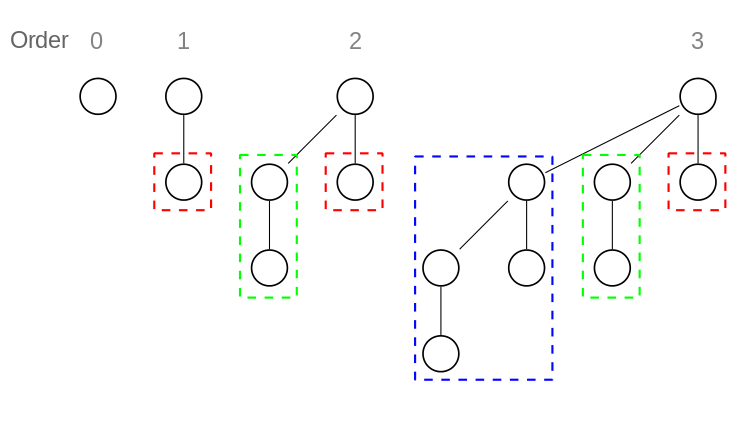
\includegraphics[width=0.75\textwidth]{binomialtree_orders}
			\caption{Verschillende ordes van binomiaalbomen.}
			\label{fig:binomialtree_orders}
		\end{figure}

		De \underline{operaties} op een binomiaalqueue:
		\begin{itemize}
			\item \textbf{Minimum vinden}: Overloop de wortel van elke binomiaalboom. Het minimum kan ook gewoon bijgehouden worden.
			\item \textbf{Samenvoegen}: Tel de bomen met dezelfde hoogte bij elkaar op, $B_h + B_h = B_{h + 1}$. Maak de wortel met de grootste sleutel het kind van deze met de kleinste. 
			\item \textbf{Toevoegen}: Maak een triviale binomiaalqueue met één knoop en voeg deze samen met de andere binomiaalqueue.
			\item \textbf{Minimum verwijderen}: Zoek binomiaalboom $B_k$ met het kleinste wortelelement. Verwijder deze uit de binomiaalqueue. Verwijder wortel van  $B_k$. Voeg beide binomiaalqueues terug samen.
		\end{itemize}

	\item \textbf{Pairing heaps}:
		\begin{itemize}
			\item Een algemene boom waarvan de sleutels voldoen aan de heapvoorwaarde.
			\item Elke knoop heeft een wijzer naar zijn linkerkind en rechterbroer (figuur \ref{fig:pairingheap_treeform} en \ref{fig:pairingheap}). Als verminderen van prioriteit moet ondersteund worden, heeft elke knoop als linkerkind een wijzer naar zijn ouder en als rechterkind een wijzer naar zijn linkerkind.
		\end{itemize}
		\begin{figure}[ht]
			\centering
			\begin{minipage}{.5\textwidth}
				\centering
				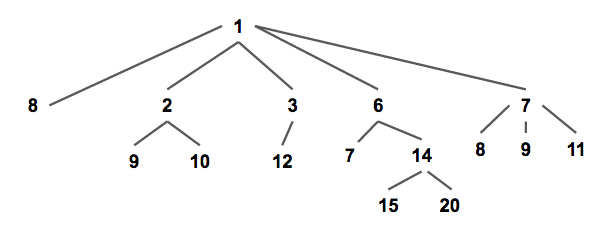
\includegraphics[width=\linewidth]{pairingheap_treeform}
				\caption{Een pairing heap in boomvorm.}
				\label{fig:pairingheap_treeform}
			\end{minipage}%
			\begin{minipage}{.5\textwidth}
				\centering
				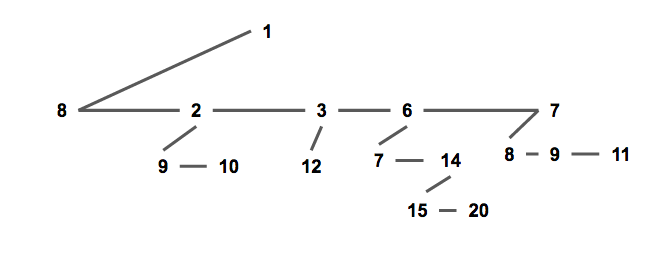
\includegraphics[width=\linewidth]{pairingheap}
				\caption{Een pairing heap.}
				\label{fig:pairingheap}
			\end{minipage}

	
		\end{figure}

		De \underline{operaties} op een pairing heap.
		\begin{itemize}
			\item \textbf{Samenvoegen}: Verlijk het wortelelement van beide heaps. De wortel met het grootste element wordt het linkerkind van deze met het kleinste element.
			\item \textbf{Toevoegen}: Maak een nieuwe pairingheap met één element, en voeg deze samen met de oorspronkelijke heap.
			\item \textbf{Prioriteit wijzigen}: De te wijzigen knoop wordt losgekoppeld, krijgt de prioriteitwijziging, en wordt dan weer samengevoegd met de oorspronkelijke heap.
			\item \textbf{Minimum verwijderen}: De wortel verwijderen levert een collectie van $c$ heaps op. Voeg deze heaps van links naar rechts samen in $O(n)$ of voeg eerst in paren toe, en dan van rechts naar links toevoegen in geamortiseerd $O(\lg n)$.
			\item \textbf{Willekeurige knoop verwijderen}: De te verwijderen knoop wordt losgekoppeld, zodat er twee deelheaps onstaan. Deze twee deelheaps worden samengevoegd.
		\end{itemize}
\end{itemize}
\part{Grafen II}
\chapter{Toepassingen van diepte-eerst zoeken}
\section{Enkelvoudige samenhang van grafen}
\subsection{Samenhangende componenten van een ongerichte graaf}
\begin{itemize}
	\item[\info] Een \textbf{samenhangende ongerichte graaf} is een graaf waarbij er een weg bestaat tussen elk paar knopen.
	\item[\info] Een \textbf{niet samenhangende ongerichte graaf} bestaat dan uit zo groot mogelijke samenhangende componenten.
\end{itemize}

\subsection{Sterk samenhangende componenten van een gerichte graaf}
\begin{itemize}
	\item[\info] Een \textbf{sterk samenhangende gerichte graaf} is een graaf waarbij er een weg tussen elk paar knopen in beide richtingen (niet perse dezelfde verbindingen) bestaat (cfr. figuur \ref{fig:sterk_samenhangende_graaf}).
	\begin{figure}[ht]
		\centering
		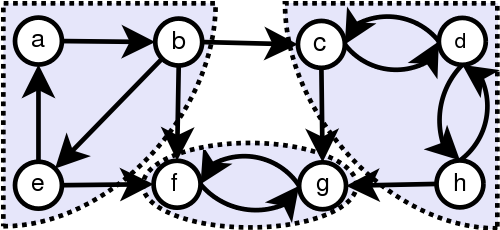
\includegraphics[width=0.5\textwidth]{img/sterk_samenhangende_graaf}
		\caption{Een sterk samenhangende graaf.}
		\label{fig:sterk_samenhangende_graaf}
	\end{figure}
				
	\item[\info] Een \textbf{zwak samenhangende gerichte graaf} is een graaf die niet sterk, maar toch samenhangend is indien de richtingen buiten beschouwing gelaten worden. Een graaf die niet sterk samenhangend is, bestaat uit zo groot mogelijke sterk samenhangende componenten. 
	\item[\info] Sommige algoritmen gaan ervan uit de een graaf sterk samenhangend is. Men moet dus eerst deze componenten bepalen, meestal via een \textbf{componentengraaf} die:
	\begin{itemize}
		\item[\info] een knoop heeft voor elk sterk samenhangend component,
		\item[\info] en een verbinding van knoop $a$ naar knoop $b$ indien er in de originele graaf een verbinding van één van de knopen van $a$ naar één van de knopen van $b$ is. 
	\end{itemize}
	\item[\alert] De componentgraaf bevat geen lussen, anders wil dit zeggen dat die knoop zelf nog opgesplitst zou kunnen worden in twee sterk samenhangende componenten.
	\item[\info] De sterk samenhangende componenten kunnen bekomen worden met behulp van diepte-eerst zoeken (Kosaraju's Algorithm):
	\begin{enumerate}
		\item Stel de omgekeerde graaf op, door de richting van elke verbinding om te keren.
		\item Pas diepte-eerst zoeken toe op deze omgekeerde graaf, waarbij de knopen in postorder genummered worden.
		\item Pas diepte-eerst zoeken toe op de originele graaf, met als startknoop de resterende knoop met het hoogste postordernummer. Het resultaat is een diepte-eerst bos, waarvan de bomen sterk samenhangende componenten zijn.
	\end{enumerate}
	\item[\info] Diepte-eerst zoeken is $\Theta(n + m)$ voor ijle en $\Theta(n^2)$ voor dichte grafen. Het omkeren van de graaf is ook $\Theta(n + m)$ voor ijle en $\Theta(n^2)$ voor dichte grafen.
\end{itemize}




\section{Dubbele samenhang van ongerichte grafen}
Twee definities:
\begin{itemize}
	\item[\info] \textbf{Brug.} Een brug is een verbinding dat, indien deze wordt weggenomen, de graaf in twee deelgrafen opsplitst. Een graaf zonder bruggen noemt men \underline{dubbel lijnsamenhangend}; als er tussen elk paar knopen minstens twee onafhankelijke wegen bestaan, dan is een graaf zeker dubbel lijnsamenhangend.
	\item[\info] \textbf{Scharnierpunt.} Een scharnierpunt is een knoop dat, indien deze wordt weggenomen, de graaf in ten minste twee deelgrafen opsplitst. Een graaf zonder scharnierpunten noemt men \underline{dubbel knoopsamenhangend} (of dubbel samenhangend). Een graaf met scharnierpunten kan onderverdeeld worden in dubbel knoopsamenhangende componenten. Als er tussen elk paar knopen twee onafhankelijke wegen bestaan, dan is de graaf dubbel knoopsamenhangend.
\end{itemize}

Scharnierpunten, dubbel knoopsamenhangende componenten, bruggen en dubbel lijnsamenhangende componenten kunnen opnieuw via diepte-eerst zoeken gevonden worden:
\begin{enumerate}
	\item Stel de diepte-eerst boom op, waarbij de knopen in postorder genummerd worden. 
	\item Bepaal voor elke knoop $u$ de laagst genummerde knoop die vanuit $u$ kan bereikt worden via een weg bestaande uit nul of meer dalende boomtakken gevolgd door één terugverbinding. 
	\item Indien alle kinderen van een knoop op die manier een knoop kunnen bereiken die hoger in de boom ligt dan hemzelf, dan is de knoop zeker niet samenhangend. De wortel is een scharnierpunt indien hij meer dan één kind in heeft. \todo{hoe bruggen vinden?}
\end{enumerate}
Diepte-eerst zoeken is $\Theta(n + m)$ voor ijle en $\Theta(n^2)$ voor dichte grafen.
\section{Eulergraaf}
Een eulercircuit is een gesloten omloop in een graaf die alle verbindingen éénmaal bevat. Een eulergraaf is een graaf met een eulercircuit, die volgende eigenschappen heeft:
\begin{itemize}
	\item De graaf is knoopsamenhangend.
	\item De graad van elke knoop is even.
	\item De verbindingen kunnen onderverdeeld worden in lussen, waarbij elke verbinding slechts behoort tot één enkel lus.
\end{itemize}

\chapter{Kortste Afstanden II}
\section{Kortste afstanden vanuit één knoop}
\subsection{Algoritme van Bellman-Ford}
Dit algoritme werkt voor verbindingen met negatieve gewichten, iets wat het algoritme van Dijkstra niet kon. Het algoritme is dan natuurlijk ook trager. \accentuate{(Dijkstra gebruikt het feit dat indien een pad naar A $\rightarrow$ C bestaat, er geen korter pad A $\rightarrow$ B $\rightarrow$ C kan zijn, daarom is het algoritme performant, maar er mogen dus geen negatieve verbindingen zijn. Indien B negatief zou zijn dan klopt Dijkstra niet.)}.

\begin{itemize}
	\item [\good] Werkt voor negatieve verbindingen.
	\item [\good] Geen globale kennis nodig van heel het netwerk, zoals bij Dijkstra, maar slechts enkel de buren van een bepaalde knoop. Daarom gebruiken routers Bellman-Ford (distance vector protocol).
	\item [\alert] Zal niet stoppen indien er een negatieve lus in de graaf zit, aangezien het pad dan zal blijven dalen tot $-\infty$. 
\end{itemize}

Het algoritme berust op een belangrijke eigenschap: Indien een graaf geen negatieve lussen heeft, zullen de kortste wegen evenmin lussen hebben en hoogstens $n - 1$ verbindingen bevatten. Hieruit kan een recursief verband opgesteld worden tussen de kortste wegen met maximaal $k$ verbindingen en de kortste wegen met maximaal $k - 1$ verbindingen.
$$d_i(k) = \min(d_i(k - 1), \min\limits_{j \in V} (d_j(k - 1) + g_{ij}))$$
met
\begin{itemize}
	\item $d_i(k)$ het gewicht van de kortste weg met maximaal $k$ verbindingen vanuit de startknoop naar knoop $i$,
	\item $g_{ij}$ het gewicht van de verbinding $(j, i)$,
	\item $j \in V$ elke buur $j$ van $i$.
\end{itemize}




Er bestaan \underline{twee goede implementaties}:
\begin{enumerate}
	\item \begin{itemize}
		\item [\info] Niet nodig om in elke iteratie alle verbindingen te onderzoeken. Als een iteratie de voorlopige kortste afstand tot een knoop niet aanpast, is het zinloos om bij de volgende iteratie de verbindingen vanuit die knoop te onderzoeken.
		\item [\info] Plaats enkel de knopen waarvan de afstand door de huidige iteratie gewijzigd werd in een wachtrij.
		\item [\info] Enkel de buren van deze knopen worden in de volgende iteratie getest.
		\item [\info] Elke buur moet, indien hij getest wordt en nog niet in de wachtrij zit, ook in de wachtrij gezet worden.
	\end{itemize}
	\item \begin{itemize}
		\item[\info] Gebruik een deque in plaats van een wachtrij.
		\item[\info] Als de afstand van een knoop wordt aangepast, en als die knoop reeds vroeger in de deque zat, dant voegt men vooraan toe, anders achteraan.
		\item[\alert] Kan in bepaalde gevallen zeer inefficiënt uitvallen.
	\end{itemize}

\end{enumerate}

\section{Kortste afstanden tussen alle knopenparen}
\begin{itemize}
	\item[\info] Voor dichte grafen $\rightarrow$ Floyd-Warshall (Algoritmen I).
	\item[\info] Voor ijle grafen $\rightarrow$ Johnson.
\end{itemize}
\subsection{Het algoritme van Johnson}
\begin{itemize}
	\item[\info] Maakt gebruik van Bellman-Ford en Dijkstra.
	\item[\info] Omdat we Dijkstra gebruiken, moet elk gewicht positief worden. 
	\begin{enumerate}
		\item Breidt de graaf uit met een nieuwe knoop $s$, die verbindingen van gewicht nul krijgt met elke andere knoop.
		\item Voer Bellman-Ford uit op de nieuwe graaf om vanuit $s$ de kortste afstand $d_i$ te bepalen tot elke originele knoop $i$.
		\item Het nieuwe gewicht $\hat{g}_{ij}$ van een oorspronkelijke verbinding $g_{ij}$ wordt gegeven door: 
		$$\hat{g}_{ij} = g_{ij} + d_i - d_j$$ 
	\end{enumerate}
	\item[\info] Het algoritme van Dijkstra kan nu worden toegepast op elke originele knoop, die alle \underline{kortste wegen} zullen vinden. Om de \underline{kortste afstanden} te bepalen moeten de originele gewichten opgeteld worden op deze wegen.
	\item[\info] Dit algoritme is $O(n(n + m)\lg n)$ want:
	\begin{itemize}
		\item[\info] Graaf uitbreiden is $\Theta(n)$.
		\item[\info] Bellman-Ford is $O(nm)$.
		\item[\info] De gewichten aanpassen is $\Theta(m)$.
		\item[\alert] $n$ maal Dijkstra is $O(n(n + m)\lg n)$. Dit is de belangrijkste term, al de andere termen mogen verwaarloosd worden.
	\end{itemize}
\end{itemize}

\section{Transitieve sluiting}
\underline{Sluiting} = algemene methode om één of meerdere verzamelingen op te bouwen. ('als een verzameling deze gegevens bevat, dan moet ze ook de volgende gegevens bevatten').

\begin{itemize}
	\item[\info] \textbf{Fixed point}:  Een sluiting wordt fixed point genoemd omdat op een bepaald moment verdere toepassing niets meer verandert, $f(x) = x$.
	\item[\info] \textbf{Least fixed point}: De kleinste $x$ zoeken zodat $f(x) = x$ voldaan wordt.
\end{itemize}

\underline{Transitieve sluiting} = 'Als $(a, b)$ en $(b, c)$ aanwezig zijn dan moet ook $(a, c)$ aanwezig zijn.'

\begin{itemize}
	\item[\info] Transitieve sluiting van een gerichte graaf is opnieuw een gerichte graaf, maar:
	\begin{itemize}
		\item[\info] er wordt een nieuwe verbinding van $i$ naar $j$ toegevoegd indien er een weg bestaat van $i$ naar $j$ in de oorspronkelijke graaf.
	\end{itemize}
	\item \underline{3 algoritmen:}
	\begin{enumerate}
		\item \textbf{Diepte-of breedte-eerst zoeken}: 
				\begin{itemize}
					\item[\info] Spoor alle knopen op die vanuit een startknoop bereikbaar zijn en herhaal dit met elke knoop.
					\item[\good] Voor ijle grafen $\rightarrow \Theta(n(n + m))$.
					\item[\alert] Voor dichte grafen $\rightarrow \Theta(n^3)$.
				\end{itemize}
		\item \textbf{Met de componentengraaf}:
				\begin{itemize}
					\item[\info] Interessant wanneer men verwacht dat de transitieve sluiting een dichte graaf zal zijn, want dan zijn veel knopen onderling bereikbaar, zodat er veel sterk samenhangende componenten zijn. Die kunnen in $\Theta(n + m)$ bepaald worden.
					\item[\info] Maak dan de componentengraaf (kan in $O(n + m))$.
					\item[\info] Als nu blijkt dat component $j$ beschikbaar is vanuit component $i$, dan zijn alle knopen van $j$ beruikbaar vanuit knopen van $i$.
				\end{itemize}
		\item \textbf{Het algoritme van Warshall}:
				\begin{itemize}
					\item[\info] Maak een reeks opeenvolgende $n \times n$ matrices $T^{(0)},T^{(1)},...,T^{(n)}$ die logische waarden bevat.
					\item[\info] Element $t_{ij}^{(k)}$ duidt aan of er een weg tussen $i$ en $j$ met mogelijke intermediaire knopen $1, 2, ..., k$ bestaat.
					\item[\info] Bepalen opeenvolgende matrices:
					$$t_{ij}^{(0)} = 
					\begin{cases}
						\hbox{onwaar} & \hbox{als } i \neq j \hbox{ en } g_{ij} = \infty\\
						\hbox{waar}   & \hbox{als } i = j \hbox{ of } g_{ij} < \infty
					\end{cases}$$
					en
					$$
						t_{ij}^{(k)} = t_{ij}^{(k - 1)} \hbox{ OF } \big(t_{ik}^{(k - 1)} \hbox{ EN } t_{kj}^{(k - 1)}\big) \qquad \hbox{voor } 1 \leq k \leq n
					$$
				\end{itemize}
				$T^{(n)}$ is de gezochte burenmatrix.
	\end{enumerate}
\end{itemize}


\chapter{Stroomnetwerken}
\begin{itemize}
	\item Gerichte graaf met twee speciale knopen: \underline{producent} en \underline{verbruiker}.
	\item Producent levert een bepaald materiaal aan verbruiker via de gerichte verbindingen van de graaf.
	\item Elke verbinding heeft een capaciteit $c(i, j)$ dat positief is, en de stroom $s(i, j)$ dat er door loopt ($0 \leq s(i, j) \leq c(i, j)$). 
	\item Verbindingen die niet bestaan, worden toch voorgesteld als een verbinding, maar met $c = 0$, zodat er geen stroom kan doorlopen. Dit maakt implementaties eenvoudiger.
	\item Een knoop bevat geen capaciteit, en kunnen hierdoor niets opslaan.
\end{itemize}
\section{Maximalestroomprobleem}
= zoveel mogelijk materiaal van producent naar verbruiker laten stromen, zonder de capaciteit van de verbinding te overschrijden.
\begin{itemize}
	\item [\info] Methode van \textbf{Ford-Fulkerson} \accentuate{('methode' aangezien manier om vergrotende paden te zoeken ontbreekt).}
	\item [\info] Iteratieve methode. Bij elke iteratie neemt netstroom vanuit producent toe.
	\item [\info] Stel de verzameling van knopen $K$, dan is de totale nettostroom $f$ uit de producent $p$ \accentuate{(De som van het materiaal dat toekomt min het materiaal dat weggaat van elke knoop)}. 
		$$f = \sum_{j \in K} (s(p, j) - s(j, p))$$
	\item [\info] De stroomverdeling is het geheel van alle stromen voor alle mogelijke knopenparen. 
	\item [\info] Het restnetwerk is een nieuw netwerk dat verkregen wordt door uit de huidige stroomverdeling een overzicht op te stellen van de mogelijke stroomtoename tussen elk paar knopen. Het restnetwerk bevat dezelfde knopen, maar niet noodzakelijk dezelfde verbindingen en capaciteit.
\end{itemize}
Het algoritme verloopt als volgt:
\begin{enumerate}
	\item Initiële stroomverdeling is nul. Het restnetwerk is initieël de volledige graaf.
	\item Bij elke iteratie wordt de huidige stroomverdeling en de verschillende capaciteiten gebruikt om een restnetwerk op te stellen.
	\item In dit restnetwerk wordt een vergrotend pad gezocht: een weg van producent naar verbruiker die nog meer stroom tussen beide toelaat.
	\item Als er geen vergrotende paden kunnen gevonden worden, stopt de iteratie, en zal de netwerkstroom maximaal zijn.
\end{enumerate}
https://www.youtube.com/watch?v=Tl90tNtKvxs



Hoe gaan we vergrotende weg zoeken? 
\begin{itemize}
	\item \textbf{Performantie afhankelijk van de capaciteiten}
		\begin{itemize}
			\item Stel dat alle capaciteiten geheel zijn en $C$ de grootste capaciteit voorstelt. Restnetwerk bepalen is $O(m)$, en daarin diepte-eerst of breedte-eerst zoeken naar een vergrotend pad is ook $O(m)$. Aantal iteraties in Ford-Fulkerson is $O(nC)$, dus totale performantie is $O(nmC)$, wat \underline{niet performant is voor grote $C$}.
			\item Neem de het vergrotend pad die de grootste stroomtoename mogelijk maakt, dan wordt het aantal iteraties $O(m\lg C)$ \accentuate{(zonder bewijs)}. Om die weg te vinden volstaat een kleine aanpassing aan het algoritme van Dijkstra: kortste afstand vervangen door grootste capaciteit, zodat de iteratiestap $O(m \lg n)$ \accentuate{(van Dijkstra)} is. De totale performantie is nu $O(m^2 \lg C \lg n)$
			\item Een vergrotende weg bepalen die een stroomtoename van minsten $c$, de cut-off, eenheden toelaat, of besluiten dat deze weg niet bestaat, kan in $O(m)$. Indien geen enkele weg meer gevonden wordt, dan is de minimale snedecapaciteit van het restnetwerk lager dan $mc$. Halveer $c$ en gaan opnieuw op zoek, maar nu naar verbindingen die de helft van de oorspronkelijke $c$ kunnen bevatten. Begin met ondergrens $c = 2^{\lfloor \lg C \rfloor}$, deze in elke fase halveren, en eindigen met één, dan wordt de maximale stroom bereikt met $O(m \lg C)$ iteraties.
		\end{itemize}
	\item \textbf{Performantie onafhankelijk van de capaciteiten}

		Deze methode is enkel \underline{interessant wanneer $C$ groot is}. Als de vergrotende weg steeds het minimum aantal verbindingen heeft, dan kan men aantonen \accentuate{(zonder bewijs)} dat de lengte van de vergrotende wegen na hoogsten $m$ iteraties stijg, en aangezien de maximale lengte $n - 1$ is, volstaan $O(nm)$ iteraties. Deze iteratiestep gebruikt ook breedte-eerst zoeken en is $O(m)$, zodat de totale performantie $O(nm^2)$ wordt.
\end{itemize}
\todo{tododo}

\chapter{Koppelen}
= een deelverzameling van de verbindingen waarin elke knoop hoogstens eenmaal voorkomt. Een maximale koppeling is een koppeling met het grootste aantal verbindingen. Soms hebben verbindingen ook een gewicht.
\section{Koppelen in tweeledige grafen}
Tweeledige graaf (of bipartiete graaf) = een ongerichte graaf waarbij de knopen in twee deelverzamelingen $L$ en $R$ kunnen verdeeld worden, zodat alle verbindingen steeds een knoop uit $L$ met een knoop uit $R$ verbinden.
\subsection{Ongewogen koppeling}
\begin{itemize}
\item Een knoop uit $L$ kan slechts met één knoop uit $R$ verbonden worden. Een maximale ongewogen koppeling zal zoveel mogelijk knopen uit $L$ met $R$ verbinden. 

\item Is eenvoudiger op te lossen met behulp van een stroomnetwerk. Daarom moet eerst de bipartiete graaf omgezet worden in een stroomnetwerk:
	\begin{itemize}
		\item Voer een producent $P$ in, die met alle knopen van $L$ verbonden wordt ($P \rightarrow L$).
		\item Voer een verbruiker $V$ in, die met alle knopen van $R$ verbonden wordt ($R \rightarrow V$).
		\item De oorspronkelijke verbindingen van de graaf krijgen nu een gerichte verbinding van $L$ naar $R$.
		\item De capaciteiten van elke verbinding wordt 1.
	\end{itemize}
	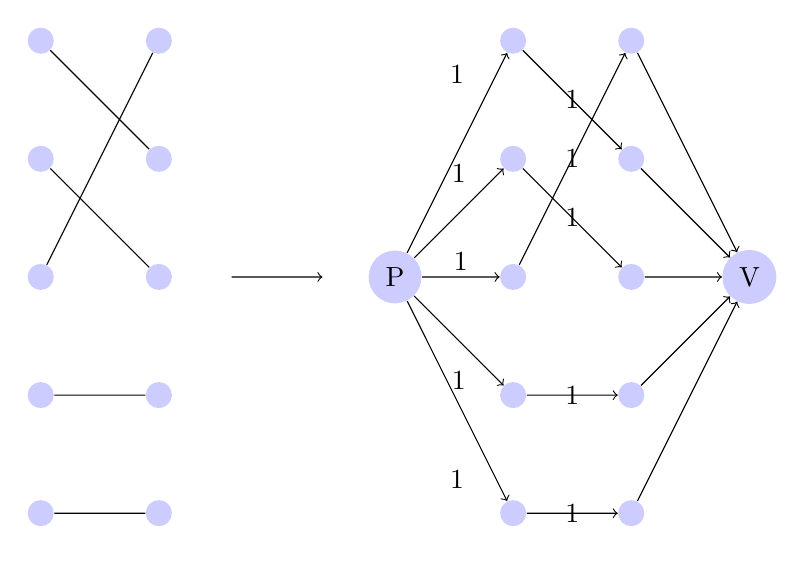
\begin{tikzpicture}[scale=1.5, every node/.style={circle, fill=blue!20},
		nocolor/.style={fill=none}
								 ]
		\node (L1) at (1, 0) {}; 
		\node (L2) at (1, -1) {};
		\node (L3) at (1, -2) {};
		\node (L4) at (1, -3) {};
		\node (L5) at (1, -4) {};

		\node (R1) at (2, 0) {}; 
		\node (R2) at (2, -1) {};
		\node (R3) at (2, -2) {};
		\node (R4) at (2, -3) {};
		\node (R5) at (2, -4) {};

		\draw (L1) -- (R2);
		\draw (L2) -- (R3);
		\draw (L3) -- (R1);
		\draw (L4) -- (R4);
		\draw (L5) -- (R5);

		\node (P) at (4, -2) {P};

		\node (A1) at (5, 0) {}; 
		\node (A2) at (5, -1) {};
		\node (A3) at (5, -2) {};
		\node (A4) at (5, -3) {};
		\node (A5) at (5, -4) {};

		\node (B1) at (6, 0) {}; 
		\node (B2) at (6, -1) {};
		\node (B3) at (6, -2) {};
		\node (B4) at (6, -3) {};
		\node (B5) at (6, -4) {};

		\node (V) at (7, -2) {V};

		\node (x) [nocolor] at (2.5, -2) {};
		\node (y) [nocolor] at (3.5, -2) {};

		\draw[->] (P) -- node[nocolor, yshift=1cm]{1} (A1);
		\draw[->] (P) -- node[nocolor , yshift=0.5cm]{1} (A2);
		\draw[->] (P) -- node[nocolor, yshift=0.2cm]{1} (A3);
		\draw[->] (P) -- node[nocolor , yshift=-0.5cm]{1} (A4);
		\draw[->] (P) -- node[nocolor , yshift=-1cm]{1} (A5);
		\draw[->] (A1) -- node[nocolor]{1} (B2);
		\draw[->] (A2) -- node[nocolor]{1} (B3);
		\draw[->] (A3) -- node[nocolor]{1} (B1);
		\draw[->] (A4) -- node[nocolor]{1} (B4);
		\draw[->] (A5) -- node[nocolor]{1} (B5);

		\draw[->] (B1)-- (V); 
		\draw[->] (B2) -- (V);
		\draw[->] (B3) -- (V);
		\draw[->] (B4) -- (V);
		\draw[->] (B5) -- (V);

		\draw[->] (x) -- (y);
	\end{tikzpicture}
\end{itemize}


\part{Strings}
\chapter{Gegevensstructuren voor strings}
\section{Digitale zoekbomen}
\begin{itemize}
	\item[\info] Analoog met gewone zoekbomen, met één verschil: de juiste deelboom wordt niet bepaald door de zoeksleutel te vergelijken met de sleutel in de knoop, maar enkel door het volgende element van de zoeksleutel (van links naar rechts). Bij de wortel gebruiken we het eerste sleutelelement, een niveau dieper het tweede sleutelelement, enz...
	\item[\info] De boom overlopen in \textbf{inorder} geeft de sleutels niet noodzakelijk in volgorde. De hoogte van de boom wordt beperkt tot het aantal bits van de grootste sleutel. Voor een groot aantal sleutels met relatief kleine bitlengte is de performantie in het slechtste geval veel beter dan die van een gewone binaire zoekboom, en vergelijkbaar met die van een rood-zwarte boom. In het gemiddelde geval is de kans op een volgend nul- of éénbit steeds gelijk, zodat er gemiddeld evenveel sleutels links als rechts komen. Daardoor is de gemiddelde hoogte van de boom $O(\lg n)$. De woordenboekoperaties zijn ook $O(\lg n)$.
	\item[\alert] De dikwijls beperkende voorwaarde is een efficiënte toegang tot de bits van de sleutels. Bovendien zijn er enkel woordenboekoperaties mogelijk.
\end{itemize}




\section{Tries}
Deze familie bomen behouden wel de sleutels in volgorde.
\subsection{Binaire tries}
\begin{itemize}
	\item[\info] Zoekweg wordt bepaald door de opeenvolgende bits van de zoeksleutel.
	\item[\info] De sleutels worden enkel opgeslagen in de bladeren, en niet in inwendige knopen.
	\item[\good] Deze boom inorder overlopen geeft wel de sleutels gerangschikt.
	\item[\good] De zoeksleutel moet niet vergeleken worden met elke knoop op de zoekweg, maar met de opeenvolgende bits.  
	\item[\info] Komen we bij een ledige deelboom terecht (nullwijzer), dan bevat de boom de zoeksleutel niet, en kan dan op deze plaats toegevoegd worden.
	\item[\info] Komen we niet bij een ledig deelboom terecht, dan bevat het blad de enige sleutel in die boom die gelijk kan zijn aan de zoeksleutel, aangezien ze dezelfde beginbits hebben.
	\item[\alert] Wanneer opgeslagen sleutels veel gelijke beginbits hebben ziujn er veel knopen met slechts één kind.
	\item[\alert] De bits van een sleutel mogen geen prefix zijn van een andere sleutel. 
	\item[\good] De structuur is onafhankelijk van de toevoegvolgorde, zodat er slechts één unieke trie is voor elke verzameling sleutels.
	\item[\info] Een trie opgebouwd uit $n$ gelijkmatige verdeelde sleutels vraagt voor zoeken of toevoegen $O(\lg n)$ bitoperaties. 
\end{itemize}


\subsection{Meerwegtries}


\section{Variabelelengtecodering}



\chapter{Zoeken in strings}
Symbolen die gebruikt worden:
\begin{table}[h]
	\centering
	\begin{tabular}{l l}
		\hline
		Symbool & Betekenis \\
		\hline 
		$\sum$ & Het gebruikte alfabet \\
		$\sum *$ & De verzameling strings van eindige lengte van letters uit $\sum$ \\
		$d$ & Aantal karakters in $\sum$ \\
		$P$ & Het patroon (naald) \\
		$p$ & Lengte van $P$ \\
		$T$ & De tekst (hooiberg) \\
		$t$ & Lengte van $T$ \\
		\hline 
	\end{tabular}
\end{table}
\section{Formele talen}
Formele taal over een alfabet = een verzameling eindige strings over dat alfabet. 

In de cursus wordt formele talentheorie beperkt tot wat in de praktijk handig is: generatieve grammatica's en reguliere uitdrukkingen.
\subsection{Generatieve grammatica's}
= Een startsymbool wordt getransformeerd tot een zin van de taal met behulp van substitutieregels. Hiervoor zijn \textbf{niet-terminale symbolen}, of kortweg niet-terminalen nodig met als notatie $\langle ... \rangle$.

$\Xi = $ De verzameling van alle strings van letters uit $\sum$ vermengd met niet-terminalen.

$\Xi* = $ de bijhorende verzameling strings.

\underline{Voorbeeld}: stel de volgende niet-terminalen (het symbool $::=$ staat voor "wordt herleidt tot"):
\begin{table}[ht]
	\centering
	\begin{tabular}{l l l}
		$\langle \textbf{S} \rangle$ & $::=$ & $\langle \textbf{AB} \rangle | \langle \textbf{CD} \rangle$ \\
		$\langle \textbf{AB} \rangle$ & $::=$ & $a\langle \textbf{AB} \rangle b | \epsilon$ \\
		$\langle \textbf{CD} \rangle$ & $::=$ & $c\langle \textbf{CD} \rangle d | \epsilon$ \\
	\end{tabular}
\end{table}
Deze grammatica definieert als formele taal de verzameling van alle strings ofwel bestaande uit een rij 'a's gevolgd door een even lange rij 'b's ofwel bestaande uit een rij 'c's gevolgd door een even lange rij 'd's. De afleiding van bijvoorbeeld de string "cccddd" wordt gegeven door
$$\langle \textbf{S} \rangle \Rightarrow  \langle \textbf{CD} \rangle  \Rightarrow  c\langle \textbf{CD} \rangle d
\Rightarrow  cc\langle \textbf{CD} \rangle dd \Rightarrow  ccc\langle \textbf{CD} \rangle ddd \Rightarrow  cccddd$$

\subsection{Reguliere uitdrukkingen}
(reguliere uitdrukking = regexp) = een string over het alfabet $\sum = \{\sigma_0, \sigma_1, ..., .\sigma_{d - 1}\}$ aangevuld met de symbolen $\emptyset$, $\epsilon$, $*$, $($, $)$ en $\underline{|}$ gedefinieerd door
\begin{table}[ht]
	\centering
	\begin{tabular}{l l l}
		$\langle \textbf{Regexp} \rangle$ & $::=$ & $\langle \textbf{basis} \rangle | \langle \textbf{samengesteld} \rangle$ \\
		$\langle \textbf{basis} \rangle$ & $::=$ & $\sigma_0 | ... | \sigma_{d - 1} | \emptyset | \epsilon$ \\
		$\langle \textbf{samengesteld} \rangle$ & $::=$ & $\langle \textbf{plus} \rangle  |  \langle \textbf{of} \rangle | \langle \textbf{ster} \rangle$ \\
		$\langle \textbf{plus} \rangle $ & $::=$ & $(\langle \textbf{Regexp} \rangle \langle \textbf{Regexp} \rangle)$ \\
		$\langle \textbf{of} \rangle $ & $::=$ & $(\langle \textbf{Regexp} \rangle \underline{|} \langle \textbf{Regexp} \rangle)$ \\
		$\langle \textbf{ster} \rangle $ & $::=$ & $(\langle \textbf{Regexp} \rangle)*$
	\end{tabular}
\end{table}
Een taal die door een regexp gedefinieerd kan worden heet een reguliere taal. 
\begin{enumerate}
	\item $\emptyset$ is een regexp, met als taal de lege verzameling.
	\item De lege string, voorgesteld als $\epsilon$, is een regexp met als taal Taal($\epsilon$) = \{$\epsilon$\}.
	\item Voor elke $a \in \sum$ is \textquotedblleft a\textquotedblright een regexp, met als taal Taal(\textquotedblleft a\textquotedblright ) = \{\textquotedblleft a\textquotedblright\}.
\end{enumerate}
Regexps kunnen gecombineerd worden:
\begin{table}[h]
	\centering
	\begin{tabular}{c c c }
		\hline
		Operatie & Regexp & Operatie op taal/talen \\
		\hline 
		Concatenatie & $(RS)$ & Taal($R$) $\cdot$ Taal($S$) \\
		of & $(R|S)$ & Taal($R$) $\cup$ Taal($S$)  \\
		Kleenesluiting & ($R$)* & Taal($R$)*
		 
	\end{tabular}
\end{table}

\section{Variabele tekst}
Zoeken van een patroon $P$ in een tekst $T$ kan op veel manieren. Wij zien volgende methoden:
\begin{itemize}
	\item Knuth-Morris-Pratt
	\item Boyer-Moore
	\item Karp-Rabinal
	\item Zoeken met automaten
	\item De Shift-AND-methode
\end{itemize}

Zie ook het bestand \texttt{Extra/zoeken\_in\_strings.pdf} voor meer methoden en uitleg.

\subsection{Eenvoudige methode}
= Voor elke positie $j$ nagaan of $P$ in $T$ voorkomt startend vanaf positie $j$, en de opeenvolgende $p$ posities. \accentuate{brol}

\subsection{Knuth-Morris-Pratt}
Eerst de definitie van een \textbf{deelstring} bepalen.

\begin{bytefield}{8}
	\bitheader{0, 1, 2, 3, 4, 5, 6, 7} \\
	\bitbox{1}{A} & \bitbox{1}{B} & \bitbox{1}{C} & \bitbox{1}{D} & \bitbox{1}{E} & \bitbox{1}{F} & \bitbox{1}{G} & \bitbox{1}{H}
\end{bytefield}

Een deelstring $(T[i], T[j])$ begint op positie $i$ en eindigt op positie $j$. Let op dat net zoals bij iterator, de positie $j$ wijst naar het element dat niet meer behoort tot de deelstring. Op het voorbeeld is de deelstring $(T[2], T[7])$ gelijk aan \texttt{CDEFG}.

De \underline{prefixfunctie} $q()$ van een string $P$ bepaalt voor elke stringpositie $i$, $1 \leq i \leq p$, de lengte van het langste prefix van $P$ met lengte kleiner dan $i$ dat we voor $i$ kunnen leggen. \accentuate{Online ga je hier vaak een andere definitie voor terugvinden, waarbij $0 \leq i \leq p$ en dus $q(0) = 0$.} 

Hieruit volgt:
\begin{itemize}
	\item $q(0) = -1$ (ongedefinieerd)
	\item $q(1) = 0$
	\item $q(i) < i$
\end{itemize}

\underline{Hoe $q(i + 1)$ berekenen?}
\begin{itemize}
	\item $q(i + 1) = q(i) + 1$ als $P[q(i)] == P[i]$
	\item Anders, $q(i + 1) = q(i) + 1$ als $P[q(q(i))] == P[i]$
	\item Anders, $q(i + 1) = q(i) + 1$ als $P[q(q(q(i)))] == P[i]$
	\item ...
	\item Als er geen enkele prefix bestaat dat we voor $i$ kunnen leggen kan verlengd worden. Dan is $q(i + 1) = 0$.
\end{itemize}

Volgende code toont de werking van de prefixfunctie.
\begin{lstlisting}
q[0] = -1
q[1] = 0
for(i = 2; i <= p; i++){
	vorig = q[i - 1]
	while(vorig > 0 && P[i - 1] != P[vorig]){
		prev = q[vorig]
	}
	if(P[i - 1] == P[vorig]){
		vorig++
	}
	q[i] = prev
}
\end{lstlisting}

Gegeven een string Q = \texttt{ANOANAANOANO}. De prefixfunctie van $Q$ komt overeen met:
\begin{lstlisting}
i = 0 1 2 3 4 5 6 7 8 9 10 11 12 
Q = A N O A N A A N O A  N  O
q = - 0 0 0 1 2 1 1 2 3  4  5  3
\end{lstlisting}

Met de prefixfunctie kan eerst een \underline{eenvoudig linear zoekalgoritme} bedacht worden:
\begin{enumerate}
	\item Stel een string samen bestaande uit $P$, gevolgd door $T$, gescheiden door een speciaal karakter $k$ dat in geen van beide voorkomt.
	
	\begin{bytefield}[bitwidth=2.4em]{15}
		\bitbox{1}{$P_0$} & \bitbox{1}{$P_1$} & \bitbox{1}{$...$} & \bitbox{1}{$P_i$} & \bitbox{1}{$...$}& \bitbox{1}{$P_{p-1}$} & \bitbox{1}{$P_p$} & \bitbox{1}{$k$} & \bitbox{1}{$T_0$} & \bitbox{1}{$T_1$} & \bitbox{1}{$...$} & \bitbox{1}{$T_j$}& \bitbox{1}{$...$}& \bitbox{1}{$T_{t-1}$} & \bitbox{1}{$T_t$}
	\end{bytefield}

	\item Bepaal nu de prefixfunctie van deze nieuwe string. Dit vereist een lineaire tijd $\Theta(t + p)$.
	\item Wanneer de prefixwaarde van een positie $i$ in deze string gelijk is aan $p$, werd $P$ gevonden, beginnend bij index $i - p$ in $T$.

\end{enumerate}

Een beter algoritme is echter dat van \underline{Knuth-Morris-Pratt}.
\begin{enumerate}
	\item 
\end{enumerate}



\subsection{Boyer-Moore}

\subsection{Karp-Rabinal}

\subsection{zoeken met automaten}

\subsection{De Shift-AND-methode}
= bitgeoriënteerde methode, die zeer efficiënt werkt voor kleine patronen, en eenvoudig kan uitgebreid worden om patronen te zoeken waarin fouten zitten.

De methode werkt als volgt:
\begin{enumerate}
	\item Stel een tabel $S$ op, die $d$ (de grootte van het alfabet) bitpatronen bevat. Bijvoorbeeld: Indien we willen zoeken in de tekst die bestaat uit karakters uit de Extended ASCII standaard. Deze standaard bevat 256 karakters. De tabel $S$ zal 256 bitpatronen bevatten. Enkel de karakters die in het patroon voorkomen zullen een bitpatroon verschillend van 0 hebben. Een bit $i$ van het bitpatroon voor karakter $k$ wordt aangezet indien $k$ voorkomt op positie $i$ in $P$. 
	
	Pseudocode:
	\begin{lstlisting}
i <- 0
zolang i < p
	Bitpatroon <- S[P[i]]
	Zet bit i van bitpatroon op 1
	i++
	\end{lstlisting}

	Een specifiek bit op 1 zetten kan via een OF operatie met het huidige bitpatroon en een bitpatroon die op positie $i$ enkel deze bit op 1 staan heeft.

	Stel dat $P = $ mijnnaald, dan ziet de overeenkomstige tabel S er uit zoals tabel \ref{table:shiftand}.
	\begin{table}[ht]
		\centering
		\begin{tabular}{l l}
			S['a'] & 00000110000000000000000000000000 \\
			S['d'] & 00000000100000000000000000000000 \\
			S['i'] & 01000000000000000000000000000000 \\
			S['j'] & 00100000000000000000000000000000 \\
			S['l'] & 00000001000000000000000000000000 \\
			S['m'] & 10000000000000000000000000000000 \\
			S['n'] & 00011000000000000000000000000000 \\	
		\end{tabular}
		\caption{Tabel $S$ voor $P = $ mijnnaald.}
		\label{table:shiftand}
	\end{table}
	De overige plaatsen hebben uiteraard allemaal een bitpatroon van 0. 
	\item \underline{Hoe kan hiermee gezocht worden in $T$?}
	
	Stel een bitpatroon $R$ op, waarvan alle bits onwaar zijn. Stel ook een bitpatroon $M$ op, waarvan slechts één bit waar is, namelijk het bit op $p - 1$. Elk karakter $T[j]$ moet nu overlopen worden. Op basis van $j$ bouwen we een nieuwe $R$, $R_{j + 1}$ op  als volgt:
	$$R_{j + 1} = (\hbox{Schuif}(R_j)\;\hbox{OF}\;Bitpatroon(1))\;\hbox{EN}\;S[T[j + 1]]$$
	De vorige $R$ waarde wordt eerst 1 positie naar rechts geschoven. Aangezien dit een nulbit vooraan zal toevoegen, moet hier ook nog een OF operatie gedaan worden zodat het bit dat vooraan staat 1 wordt. Dit wordt gevolgd door een EN operatie met het bitpatroon voor karakter $T[j + 1]$. Er zijn dan drie gevallen:
	\begin{itemize}
		\item Het bitpatroon van $T[j + 1]$ is 0. De nieuwe $R$ krijgt terug een nulbitpatroon, wat neerkomt dat er terug in het begin van het patroon zal gezocht worden.
		\item Het bitpatroon van $T[j + 1]$ is verschillend van 0, maar de positie $i$ van het meest rechtste éénbit van $R$ heeft een nulbit in $T$ op positie $i$. Dit wil zeggen dat $R$ opnieuw bitpatroon 0 krijgt, en er opnieuw in het begin van het patroon moet gezocht worden.
		\item Het bitpatroon van $T[j + 1]$ is verschillend van 0, en de positie $i$ van het meest rechtste éénbit van $R$ heeft ook een éénbit in $T$ op positie $i$. Dit wil zeggen dat het patroon matcht met de huidige waarde $T[j + 1]$, en er dus verder in het patroon (door de bitshift naar rechts uit te voeren) wordt gezocht.
	\end{itemize}

	Wanneer $R = M$, dan wil zeggen dat het patroon gevonden is in $T$. $R$ wordt dan opnieuw geinitialiseerd tot een nulbitpatroon, en kan er verder gezocht worden in $T$.

	Pseudocode:
	\begin{lstlisting}
R <- bitpatroon 0
M <- bitpatroon waarbij bit p - 1 waar is
j <- 0
zolang j < t 
	R <- (Schuif(R) OF Bitpatroon 1) EN S[T[j]]
	if(R EN M){
		patroon gevonden
	} 
	j++
	\end{lstlisting}
\end{enumerate}

<<<<<<< HEAD
=======
\chapter{Indexeren van vaste tekst}
\begin{itemize}
	\item[\info] Voorbereidend werk op de tekst, zodat zoeken in tekst tot $O(p)$ kan gereduceerd worden.
	\item[\info] Opslaan van de \underline{suffixen} van de tekst in een bepaalde gegevensstructuur.
	\item[\info] Als het patroon in de tekst voorkomt, moet het een \underline{prefix} zijn van één van die suffixen.
	\item[\info] Om te vermijden dat een suffix een prefix vaneen ander suffix zou zijn, sluiten we de tekst af met een speciaal karakter.
	\item[\info] $suff_i = $ suffix dat begint op lokatie $i$.   

\end{itemize}
\section{Suffixbomen}
\begin{itemize}
	\item[\alert] Gebruik geen meerwegstrie. De zoektijd zou wel beperkt worden door sleutellengte $p$, maar toevoegen is $O(t^2)$ en het neemt onnodig veel geheugen in beslag. 
	\item[\info] De suffixboom bevat alle suffixen van dezelfde tekst.
	\item[\info] Het is verwant met de patriciatrie, maar met volgende wijzigingen:
		\begin{itemize}
			\item[\info] In plaats van \emph{suff}$_i$ op te slagen, volstaat de beginindex $i$. De tekst moet wel bijgehouden worden.
			\item[\info]  \todo{dunno}
			\item[\info] Er wordt een staartpointer opgenomen in elke inwendige knoop, die constructie en sommige toepassingen veel sneller maakt. 
		\end{itemize}
	\item[\info] $staart(abcd) = bcd$. De staart van een string is de string bekomen door het eerste karakter te verwijderen.
	\item[\info] We starten met een lege suffixboom en voegen elke keer één karakter van $T$ toe, zodat we na $k$ iteraties suffixen hebben van de string $T[0] ... T[k - 1]$, zonder afsluitteken.

	Na $k$ iteraties is er een kleinste index $i$, die gelijk is aan $k$, zodanig dat het incomplete \emph{suff}$_i$ een prefix is van een vorig suffix. Dan geldt:

	\begin{enumerate}
		\item Alle suffixen \emph{suff}$_j$ waarvoor $j < i$ zijn geen prefix en worden aangeduid als een blad.
		\item Alle suffixen \emph{suff}$_j$ met $j\geq i$ zijn een prefix van een andere string en zijn niet zichtbaar in de suffixboom. \emph{suff}$_i$ noemen we het actieve suffix.
	\end{enumerate}

	\underline{Wat als we $T[k]$ toevoegen?} Alle strings in de suffixboom moet met dit karakter verlengd worden en het karakter $T[k]$ moet toegevoegd worden in de boom, tenzij dit karakter al eerder in de string zat, want dan is deze string een prefix dat we niet te zien krijgen.
	\begin{enumerate}
		\item Voor suffixen die aangeduid worden door een blad moeten we niets doen.
		\item Overloop de strings af die een prefix waren, in orde van dalende lengte. Er zijn er nul of meer die door dit extra karakter geen prefix meer zijn. Die moeten een blad krijgen, waarna we naar het volgende suffix gaan.
	\end{enumerate}

	\item[\info] De toevoegoperatie van hierboven voegt steeds een blad toe, en springt verder naar de volgende impliciet aanwezige suffix, zodat de toevoegoperatie $O(t)$ is. 

	Om dit te bereiken houden we een pointer bij naar de laatst toegevoegde inwendige knoop en een pointer naar het actieve punt.
	
	Het actieve punt is de laatste explicite inwendige knoop die we tegenkomen als we het actieve suffix zouden zoeken in de suffixboom.


	\item[\info] \underline{Toepassingen van een suffixboom}:
	\begin{itemize}
		\item[\info] Het deelstringprobleem (Geef alle beginposities van $P$ in $T$). 

		Construeer de suffixboom voor $T$, en zoek dan de knoop die overeenkomt met $P$.
		\begin{enumerate}
			\item Bestaat de knoop niet, dan komt $P$ niet in $T$ voor. 
			\item Bestaat de knoop wel, dan zijn de gezochte beginposities de indices bij alle bladeren die opvolgers zijn van deze knoop. 
		\end{enumerate}

		Als $P$ $k$ maal voorkomt, kan die gevonden worden in $O(p + k)$ want elke deelboom heeft hoogstens $k - 1$ inwendige knopen.
		\item[\info] Langste gemeenschappelijke deelstring (Gegeven een verzameling van $k$ verschillende strings $S = \{s_1, s_2, ..., s_k\}$, met totale lengte $t$. Gezocht de langste gemeenschappelijke deelstring van al die strings.)

		Construeer een veralgemeende suffixboom, die al de suffixen bevat van al de strings uit deze verzameling. De bladeren bevatten niet enkel de beginpositie van de suffix, maar ook de string waartoe die behoort. De constructietijd voor een verzameling strings met totale lengte $t$ is $O(t)$.

		De boom wordt systematisch overlopen om de lengte van alle prefixen en het aantal verschillende strings te bepalen waarin ze voorkomen, en dus meteen ook het langste prefix dat in alle strings voorkomt. 

		Voorzie voor elke string in $S$ een verschillend afsluitkarakter, op die manier kunnen we zien tot welke string deze behoort, en behoort elk blad maar tot één string.


	\end{itemize}
	

\end{itemize}
\section{Suffixtabellen}
\section{Tekstzoekmachines}

>>>>>>> e0a834a1089a178d044438d9f8cfdda6f8cca6b1
\part{Hardnekkige problemen}
\chapter{NP}
\section{Complexiteit: P en NP}
Elk probleem wordt voorgesteld als een beslissingsprobleem, in de vorm van 'Bestaat er een ...?'.

\underline{De klasse P(olynomiaal)}: bevat alle problemen waarvan de uitvoeringstijd begrensd wordt door een veelterm in de grootte van het probleem, bij uitvoering op een realistisch computermodel.
\begin{itemize}
	\item Grootte = het aantal bits bedoeld dat nodig is om de invoergegevens in een computer voor te stellen. Deze voorstelling is compact, bevat geen overtollige informatie, en stelt getallen voor in een talstelsel met radix groter dan 1.
	\item Realistisch computermodel = heeft een polynomiale bovengrens voor het werk dat in één tijdseenheid kan verricht worden. 
\end{itemize}

Elk probleem in P wordt als efficiënt oplosbaar beschouwd.

Waarom veeltermen gebruiken, want $O(n^{100})$ is toch niet efficiënt?
\begin{enumerate}
	\item Als uitvoeringstijd niet begrensd is door een veelterm, is het niet efficiënt oplosbaar. Normaal is de graad ook beperkt (zelden meer dan twee of drie).
	\item Veeltermen zijn de kleinste klasse functies die kunnen gecombineerd worden warbij het resultaat opnieuw een veelterm is. 
\end{enumerate}

\underline{De klasse N(iet deterministisch) P(olynomiaal)}: Als het opsplitsen van een verzameling kandidaten en het controleren van één kandidaat beide in polynomiale tijd kunnen gebeuren, dan kan een niet-deterministische computer het antwoord geven in polynomiale tijd.
\begin{itemize}
	\item Niet-deterministische computer = Een computer met oneindig veel processoren, waarbij elke processor in een tijdsinterval $k$ aantal andere processoren kan aanspreken. In $t$ tijdsintervallen kunnen we $t^k$ processoren aan het werk stellen. Deze processoren werken niet samen, ze kunnen enkel hun deel van het probleem oplossen.
	\item Kandidaat = Een kandidaatoplossing voor een deelprobleem. Denk bijvoorbeeld aand sudoku; stel dat je een getal in een vakje moet plaatsen, kan je dit gewoon aan 9 processoren doorgeven en wachten op hun resultaat, sommige van deze processoren zullen op het beslissingsprobleem 'nee' antwoorden, en sommige 'ja'.
\end{itemize}

Elk probleem uit $P$ behoort dus zeker tot $NP$, want je kan gewoon het probleem aan de hoofdprocessor van de niet-deterministische computer geven. Men is er toch niet in geslaagd om aan te tonen dat de niet-deterministische computer krachtiger is dan de klassieke determinstische computer. Dit heet het $P-versus-NP$ probleem.

\underline{NP-harde problemen}: Als we een probleem $X$ kunnen reduceren naar een probleem $Y$, dan is $Y$ minstens even zwaar als $X$. Een reductie is het omvormen van het ene probleem naar een ander. Er zullen dus problemen zijn die minstens even zwaar zijn als elk NP-probleem. Deze problemen noemen we NP-hard.

\underline{NP-complete problemen}: Dit zijn NP-harde problemen die zeker in NP zitten. Een NP-complete problemen hebben een typische structuur die aan backtracking doen denken, waardoor het vaa kvrij gemakkelijk door reductie van het ene naar het andere problem over te gaan.

Indien er één NP-compleet probleem tot P zou behoren, dan behoren alle NP-complete problemen tot P. Op die manier wordt $NP = P$.

Als je kan bewijzen dat een bepaald probleem NP-compleet is, weet je dat je niet moet zoeken naar een efficiënte oplossing, maar kan je eerder gebruik maken van volgende technieken:
\begin{itemize}
	\item Als de invoer van het probleem relatief klein is, kan je toch met backtracking alle mogelijkheden doorzoeken (bv 3x3 sudoku).
	\item Misschien bestaan er efficiënte algoritmen om speciale gevallen van het probleem op te lossen.
	\item Misschien is de gemiddelde uitvoeringstijd stukken beter dan het slechtste geval.
	\item Er bestaan benaderde algoritmen, die de vereisten voor de oplossing wat relaxeren. Sommige benaderingen zijn zelf NP-compleet.
	\item Maak gebruik van efficiënte heuritische methoden. Deze geven vaak niet de optimale oplossing, maar wel vaak een goede, maar het kan ook de slechtste oplossing zijn.
\end{itemize}

\section{NP-complete problemen}
\subsection{Het basisprobleem: SAT (en 3SAT)}
Gegeven een verzameling logische variabelen $\chi = \{x_1, ..., x_n\}$ en een collectie logische uitspraken $\mathcal{F} = \{F_1, ..., F_m \}$
Elke uitspraak $F_j$ bestaat uit atomaire uitspraken $x_i$ of de inverse $\overline{x_i}$ samengevoegd met ofoperaties zoals:
$$F_1 = x_2 \vee \overline{x_5} \vee x_7 \vee x_8 \vee x_9$$.
De vraag is nu: \underline{kan men waarden toekennen aan de variabelen, zodat elke uitspraak $F_j$ waar is?} 

Dit is natuurlijk eenvoudig op te lossen met backtracking, door incrementeel waarden toe te kennen.

Er werd bewezen dat elk probleem uit NP polynomiaal kan gereduceerd worden tot het SAT probleem. 

Er is hier nog een uitbreiding op, waarbij elke uitspraak slechts 3 atomaire variabelen mag bevatten. We kunnen $F_1$ dan omvormen naar:
\begin{equation*}
	\begin{split}
		F'_1  & = x_2 \vee \overline{x_5} \vee x_n \\
		F''_1  & = \overline{x_n} \vee x_7 \vee x_m \\
		F'''_1 & = \overline{x_m} \vee x_8 \vee x_9
	\end{split}
\end{equation*}

\subsection{Graafproblemen}
\subsubsection{Vertex Cover}
\todo{les 06 december}



\end{document}


